\documentclass[12pt]{article}

\usepackage{fullpage}
\usepackage{graphicx, rotating, booktabs} 
\usepackage{times} 
\usepackage{natbib} 
\usepackage{indentfirst} 
\usepackage{setspace}
\usepackage{grffile} 
\usepackage{hyperref}
\usepackage{adjustbox}
\setcitestyle{aysep{}}


\singlespace
\title{\textbf{Appendix to Paper: Alliance Participation and Military Spending}}
%\author{Joshua Alley}
\date{}

\bibliographystyle{apsr}

\begin{document}

\maketitle 

\doublespace 



\section{Priors}

\autoref{tab:priors} summarizes the prior distributions in the multilevel model. 
All priors are weakly informative relative to the scale of the data. 
$\nu$ is the degrees of freedom for the t-distribution, and the gamma prior is the recommended default prior for STAN. 

\begin{table} % Create a table of priors.
\begin{center}
\begin{tabular}{c} 
$ p(\alpha) \sim N(0, 1)$  \\
$ p(\sigma) \sim \mbox{half-}N(0, 1) $ \\
$ p(\alpha^{yr}) \sim N(0, \sigma^{yr}) $ \\ 
$ p(\sigma^{yr}) \sim N(0, 1) $ \\
$ p(\alpha^{st}) \sim N(0, \sigma^{st}) $ \\ 
$ p(\sigma^{st}) \sim \mbox{half-}N(0, 1) $ \\ 
$ p(\sigma^{all}) \sim \mbox{half-}N(0, 1) $ \\
$ p(\beta) \sim N(0, 1) $ \\
$ p(\gamma) \sim N(0, 1) $ \\ 
$ p(\nu) \sim gamma(2, 0.1)$ 
\end{tabular} 
\caption{Summary of Priors in Multilevel Model} 
\label{tab:priors}
\end{center} 
\end{table} 


\section{Hamiltonian Monte Carlo Diagnostics}

There were no divergent iterations in either sample running 4 chains for 2,000 iterations with 1,000 warmup iterations. 
The $\hat{R}$ is less than 1.1 for all parameters in both samples. 
Trace plots in \autoref{fig:trace-all-min} and \autoref{fig:trace-all-maj} indicate good mixing of the chains for the alliance-level parameters. 
Taken together, all of this implies that the chains adequately explored the posterior distribution. 

\begin{figure}[htbp]
	\centering
		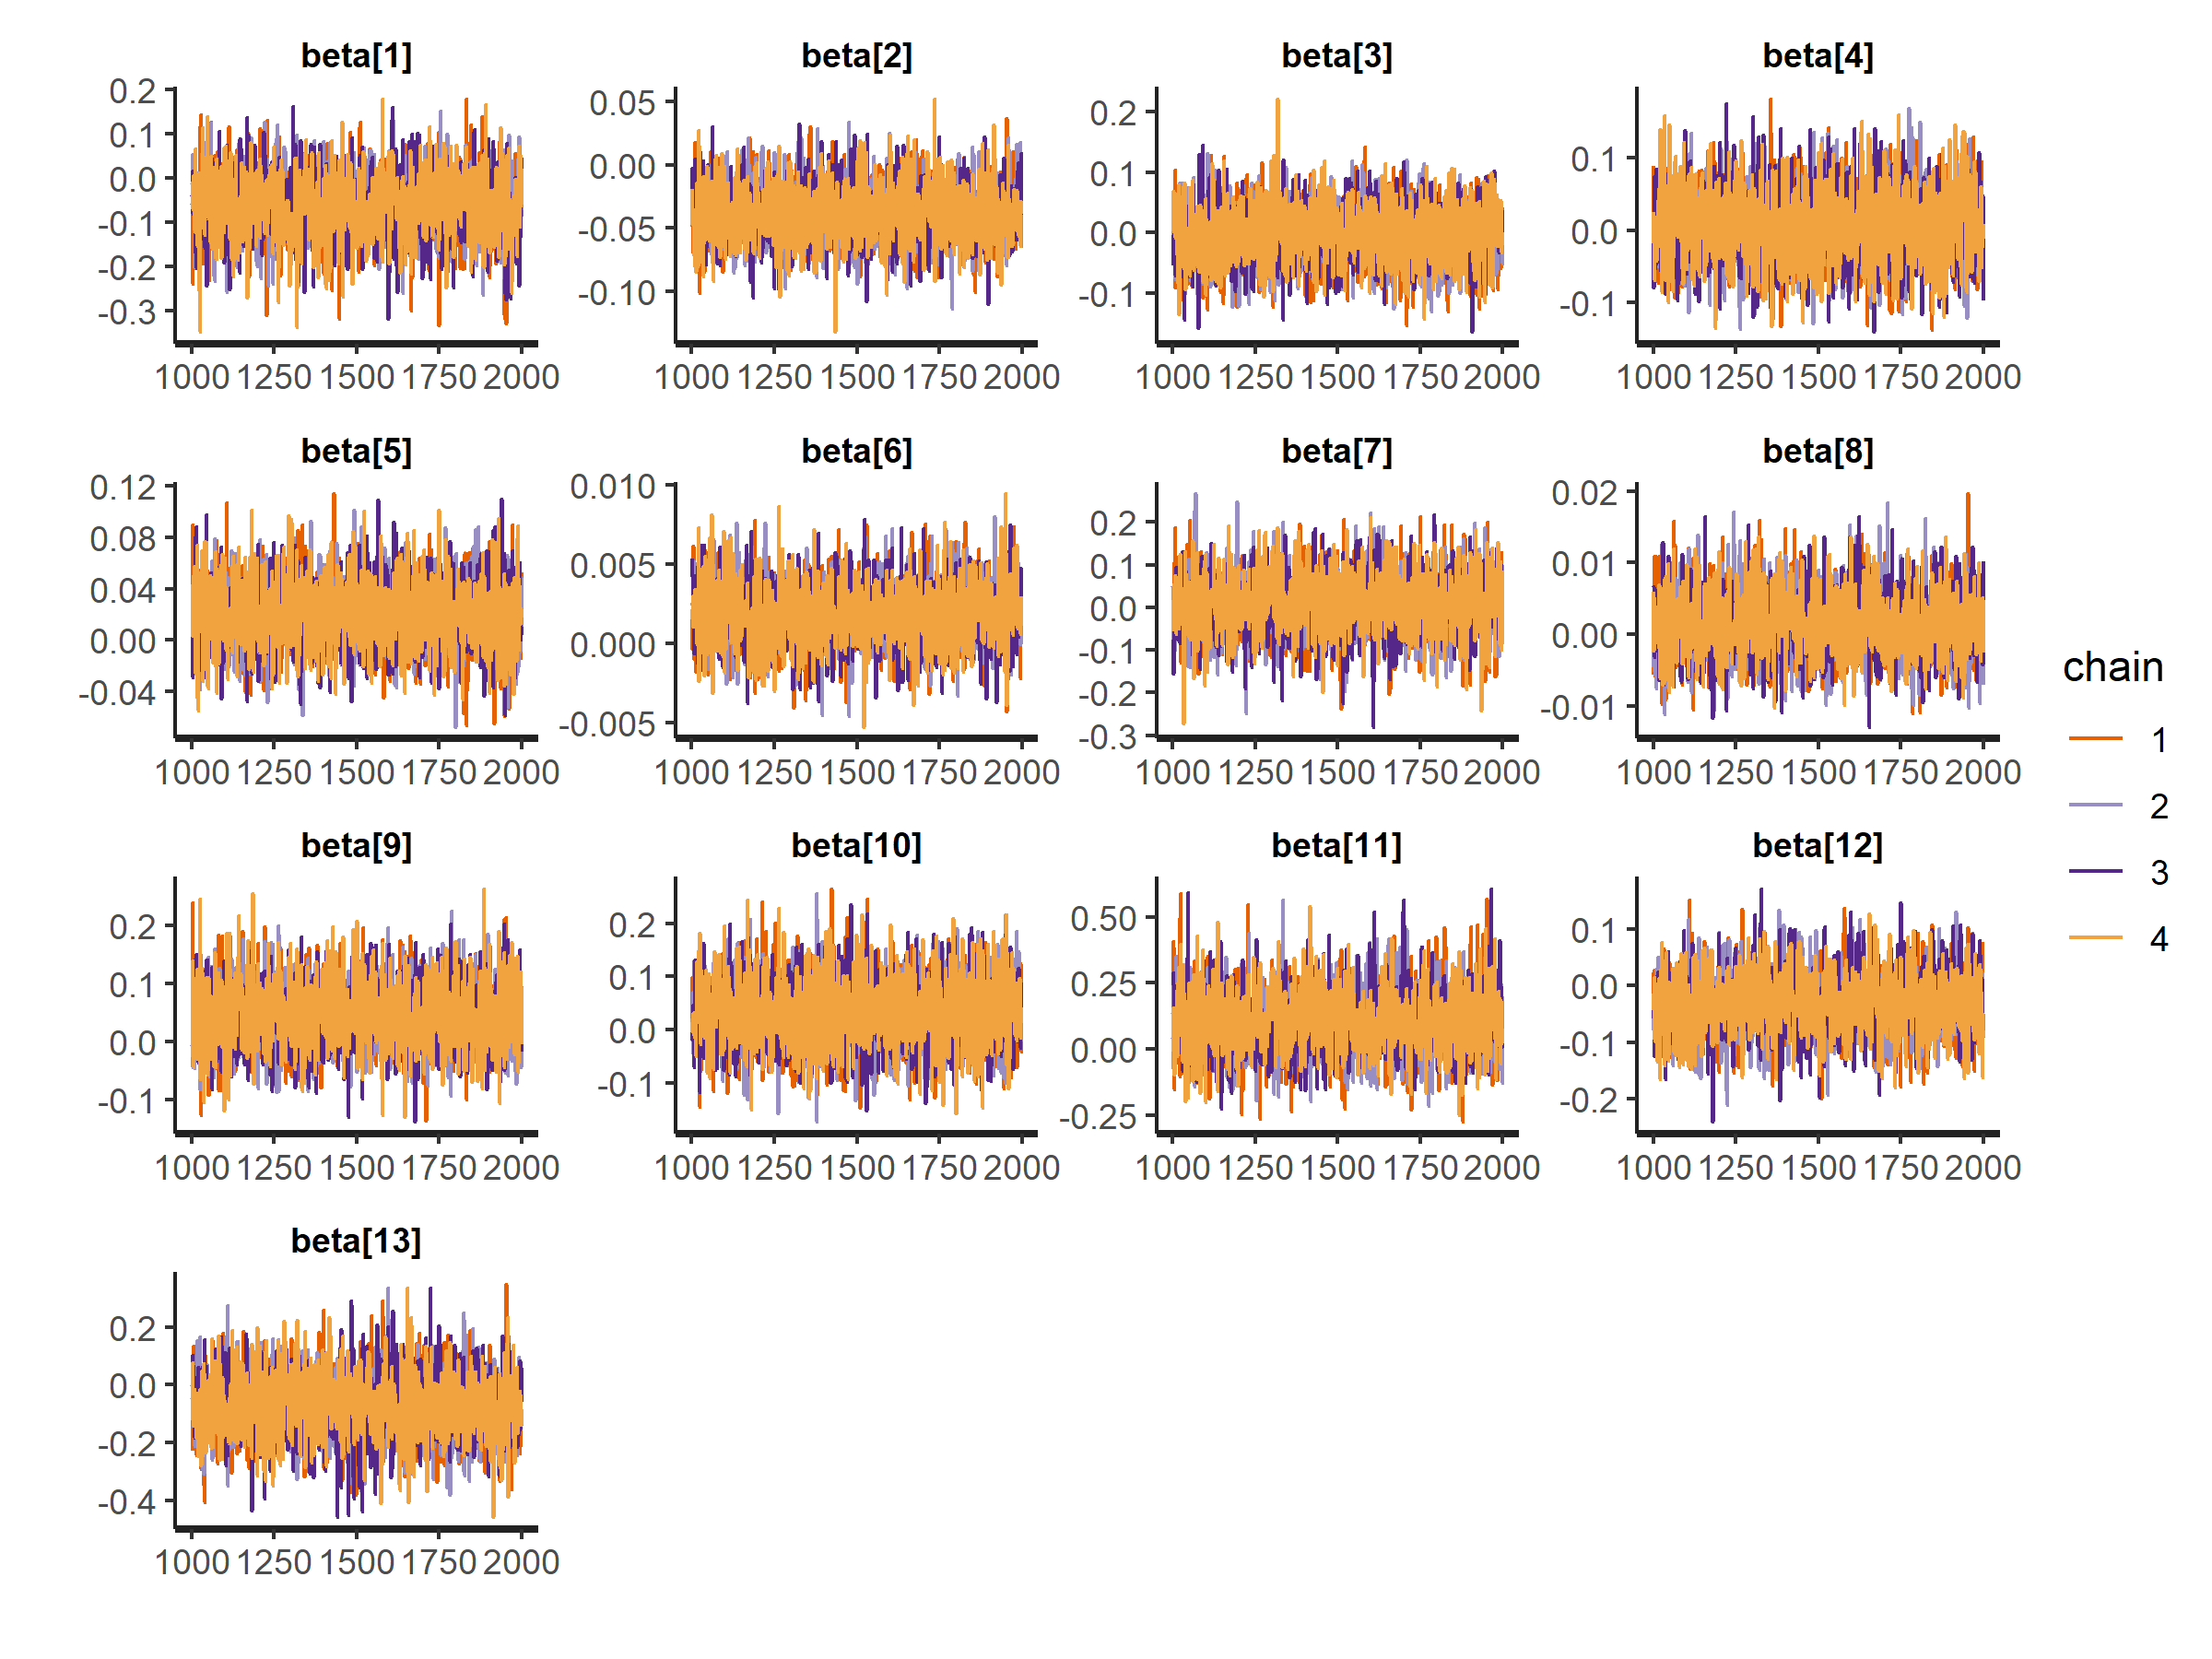
\includegraphics[width=0.95\textwidth]{trace-all-min.png}
	\caption{Traceplot of alliance level parameters in the non-major power sample.}
	\label{fig:trace-all-min}
\end{figure}


\begin{figure}[htbp]
	\centering
		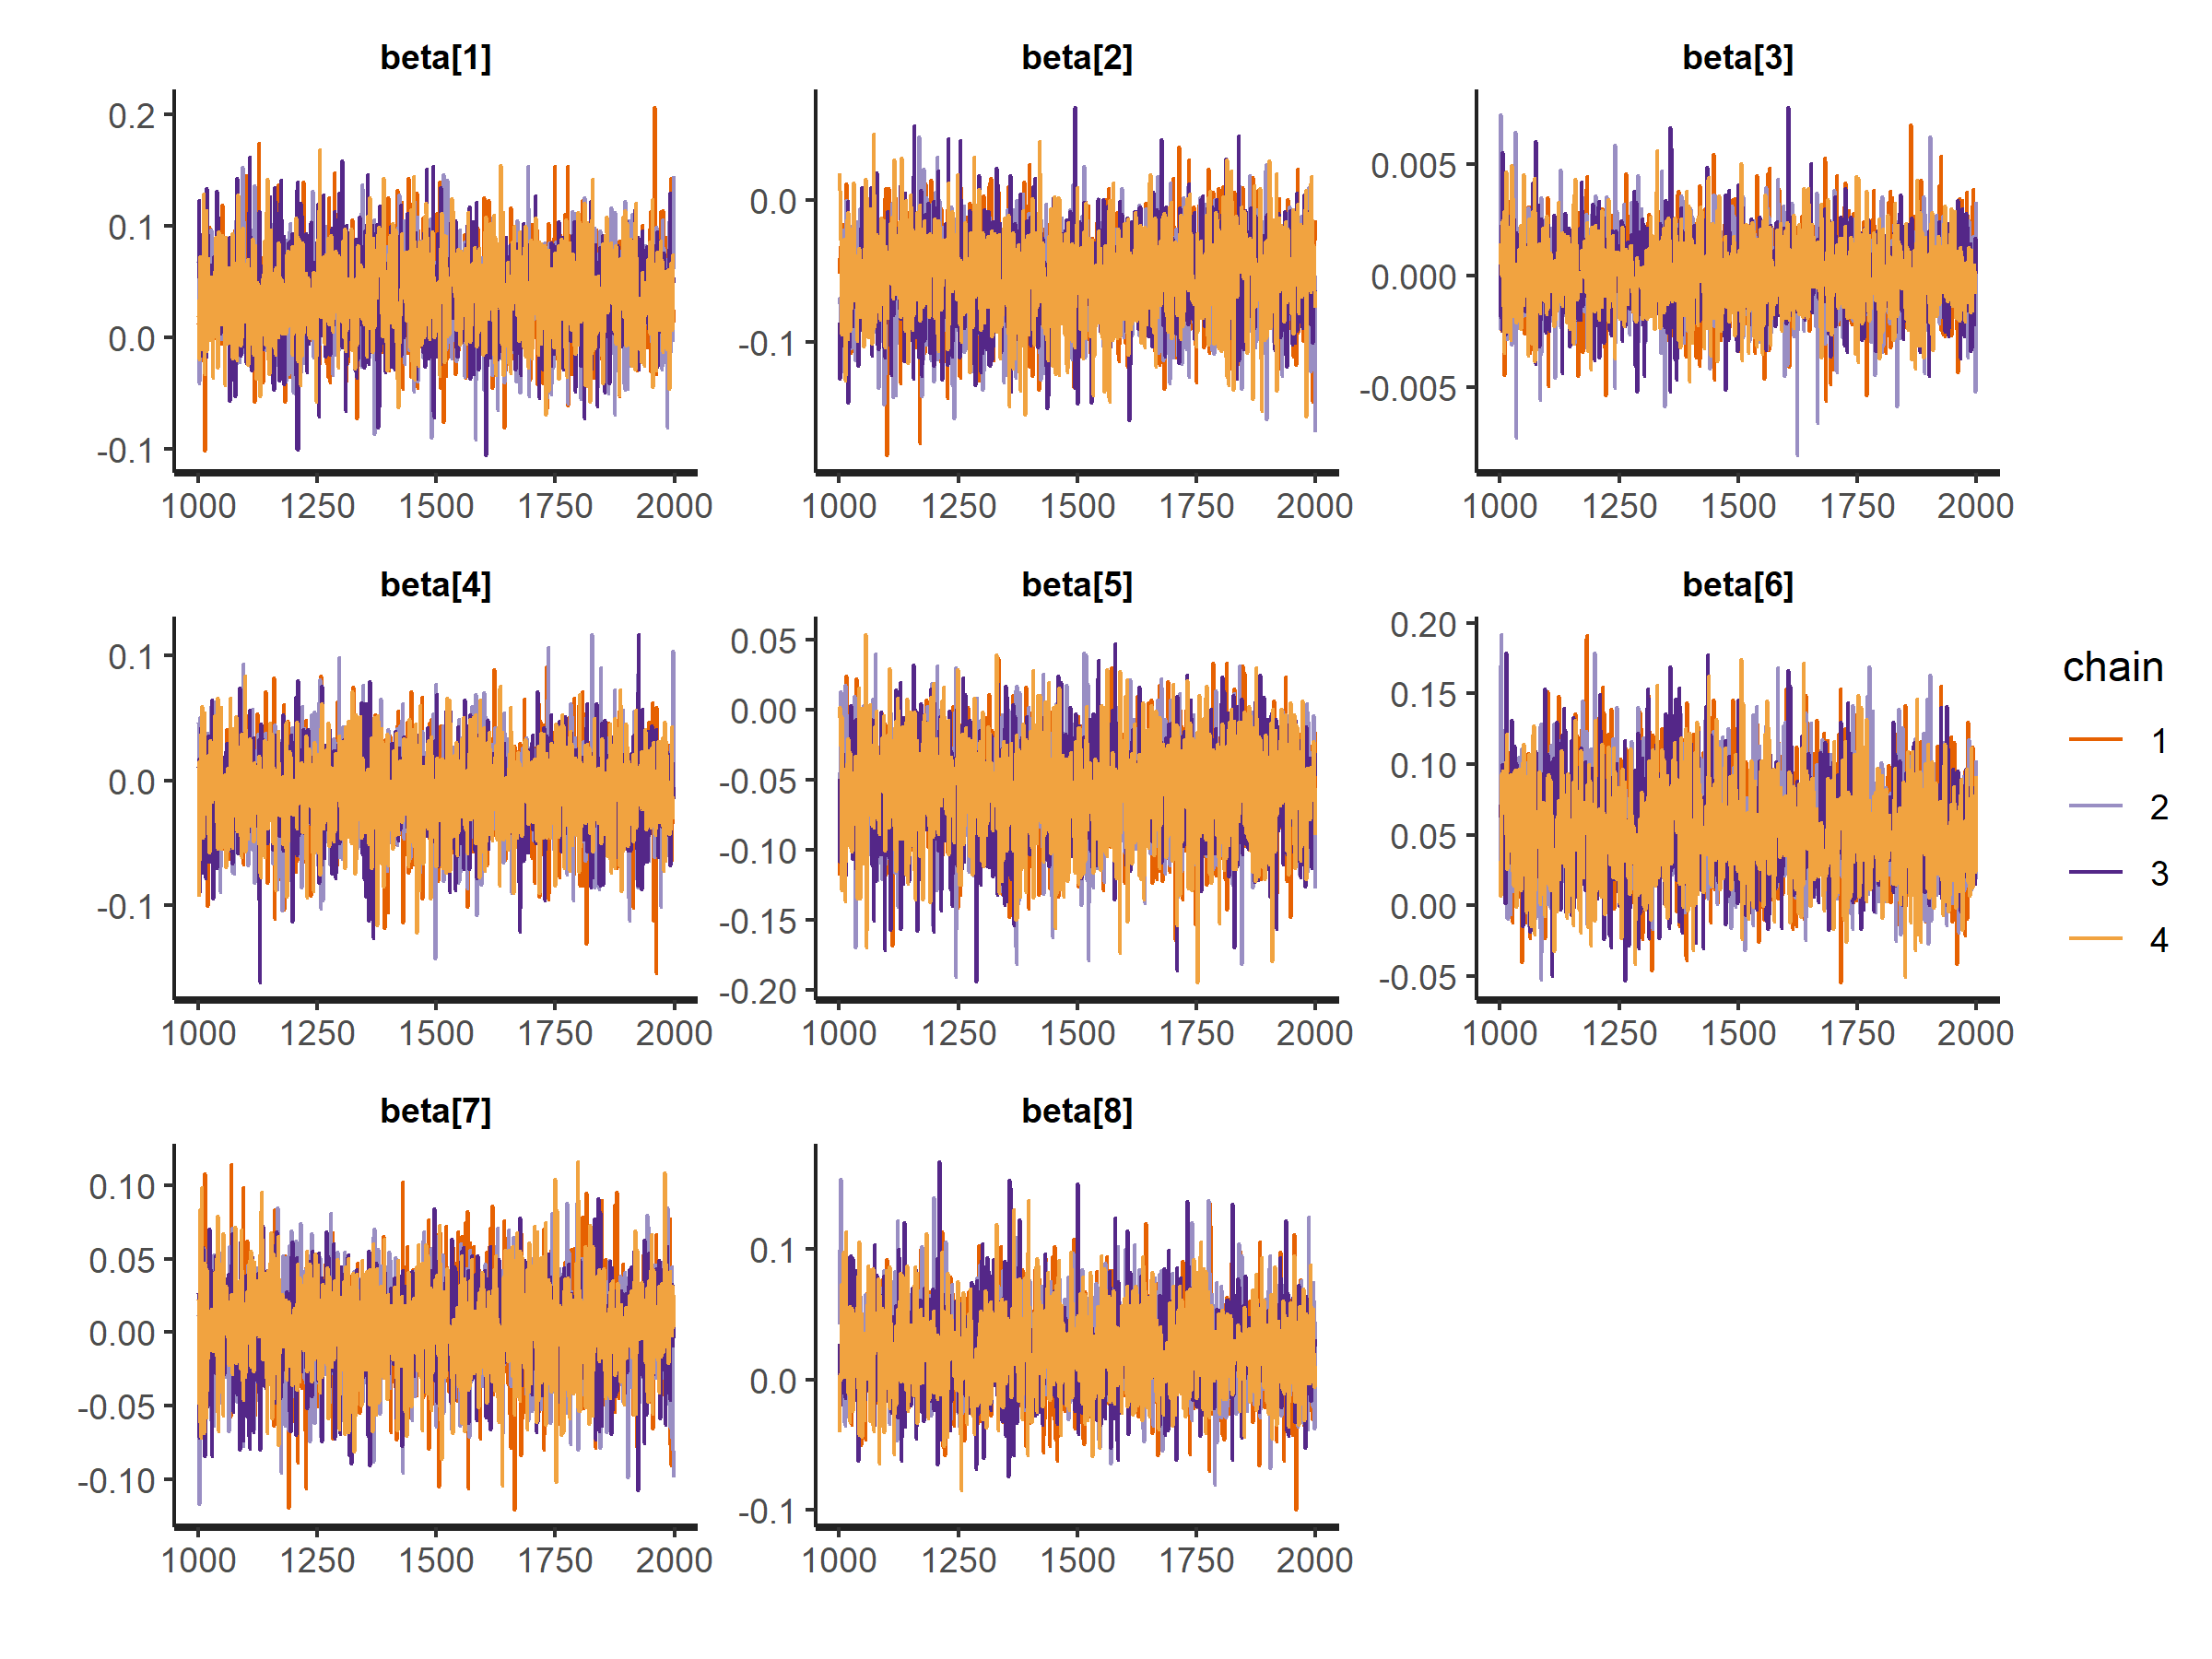
\includegraphics[width=0.95\textwidth]{trace-all-maj.png}
	\caption{Traceplot of alliance level parameters in the major power sample.}
	\label{fig:trace-all-maj}
\end{figure}


\section{Fake Data Simulation Check}


Given the complexity of the model, simulating fake data and seeing if the model can recover known parameters is another way to validate the estimates. 
Fake-data simulation is an essential aspect of model checking. 
This section summarizes results from fitting the multilevel model to fake data.


I simulated a dataset of 2000 t-distributed observations with 50 states observed for 200 years and 100 alliances. 
The outcome has a different scale than the military spending growth variable in the paper.
Thus coefficient values here will not match reported values in the paper.  
I then simulated two state and alliance level variables and a sparse matrix of state membership in alliances. 
Last, I ran the model without evaluating the likelihood, generating a posterior prediction of the outcome based on the fake data.


To check whether the model could recover known parameters, I took the 12th draw of the posterior distribution.
This draw included a simulated outcome for each observation and a set of coefficients. 
I then fit the multilevel model on the simulated outcome values and checked whether the credible intervals contained the corresponding parameter values. 
If a parameter is within the 90\% credible interval, the model captures it. 


The model recovers known parameters with a high degree of accuracy. 
As shown by \autoref{fig:beta-sim-res}, the two credible intervals of the alliance-level regression include the known values.
Credible interval coverage for the variance hyperparameters and $\gamma$ parameters is also acceptable. 


\begin{figure}[htbp]
	\centering
		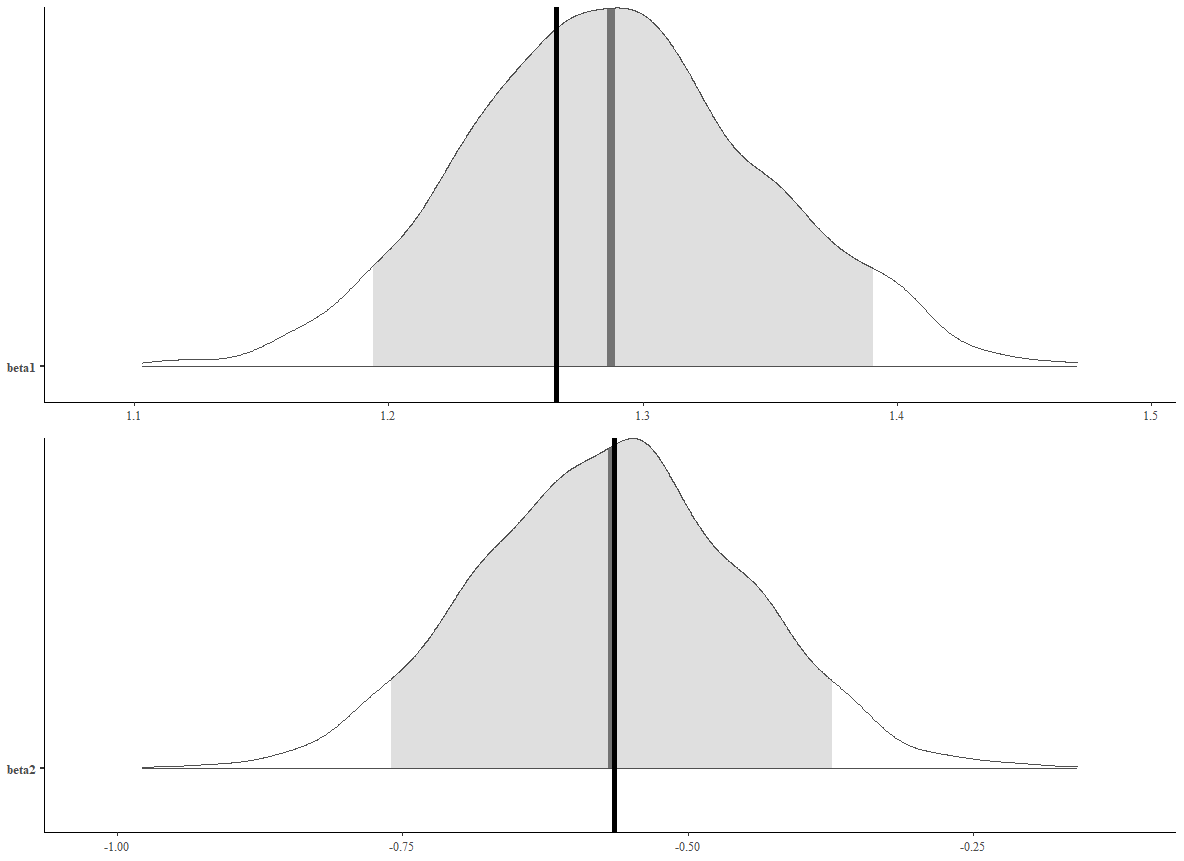
\includegraphics[width=0.95\textwidth]{beta-sim-res.png}
	\caption{Posterior distributions of $\beta$ parameters from fitting multilevel model to fake data. The black vertical line marks the known parameter value, and the grey area is the 90\% credible interval.}
	\label{fig:beta-sim-res}
\end{figure}


 
The 100 $\lambda$ parameters are harder to plot, so I offer a descriptive summary here. 
Among the $\lambda$ parameters, 93 of 100 intervals contain the known $\lambda$ value.
Given the large number of parameters and smaller sample, this is acceptable accuracy. 
Even the seven inaccurate confidence intervals were quite close--- all were within .015 of the known parameter.\footnote{Fine margins around these intervals implies that the exact number of accurate $\lambda$ intervals is very sensitive to simulation variance.}


In summary, convergence diagnostics and fake data fitting both suggest that the multilevel model is working well. 
No convergence diagnostics indicate problems exploring the posterior. 
Just as importantly, the model can recover known parameters from fake data. 
The next section provides more detail on results from the major and non-major power samples. 



\section{Posterior Intervals} 


I do not present tabular summaries of all the alliance-level parameters in the manuscript. 
The next two tables summarize the posteriors of the alliance-level parameters. 
Using a 90\% credible intervals implies there is a 90\% chance the coefficient is between the 5\% and 95\% values. 
Because Hypotheses 1 and 2 are directional, I report the positive and negative posterior probabilities in the manuscript.  
Like a one-tailed hypothesis test, the positive and negative posterior probabilities match the hypotheses better. 

\subsection{Major Powers}


\autoref{tab:alliance-level-maj} summarizes the 90\% credible intervals for the alliance parameters in the major power sample, as well as the number of effective samples and $\hat{R}$ for each marginal posterior.\footnote{I report 90\% credible intervals because 95\% interval estimates can be unstable.} 
$\sigma$ Alliances is the variance hyperparameter for the $\lambda$ estimates. 
The $\hat{R}$ statistics are all close to one, indicating convergence. 
The number of effective samples is adequate for most parameters. 


\begin{table}[ht]
\centering
\begin{tabular}{rrrrrrr}
  \hline
 & Mean & S.D. & 5\% & 95\% & Num. Eff. & $\hat{R}$ \\ 
  \hline
Constant & 0.038 & 0.038 & -0.025 & 0.102 & 3380.954 & 1.000 \\ 
  Latent Str. & -0.054 & 0.031 & -0.107 & -0.005 & 3278.923 & 1.000 \\ 
  Number Members & 0.000 & 0.002 & -0.003 & 0.003 & 4000.000 & 0.999 \\ 
  Democratic Membership & -0.009 & 0.033 & -0.065 & 0.042 & 4000.000 & 1.000 \\ 
  Wartime & -0.057 & 0.035 & -0.115 & -0.001 & 4000.000 & 1.001 \\ 
  Asymmetric & 0.053 & 0.035 & 0.001 & 0.115 & 2218.509 & 1.000 \\ 
  US Member & 0.002 & 0.031 & -0.051 & 0.051 & 4000.000 & 1.000 \\ 
  USSR Member & 0.023 & 0.033 & -0.028 & 0.079 & 4000.000 & 1.000 \\ 
  $\sigma$ Alliances & 0.066 & 0.029 & 0.019 & 0.117 & 599.081 & 1.007 \\ 
   \hline
\end{tabular}
\caption{90\% Credible intervals for major power alliance-level parameters}
\label{tab:alliance-level-maj}
\end{table}



\subsection{Non-major Powers} 

\autoref{tab:alliance-level-min} summarize the 90\% credible intervals for the alliance-level regression parameters in the non-major power sample. 
The $\hat{R}$ statistics are all close to one, indicating convergence. 
Again, the number of effective samples is adequate for all parameters.

\begin{table}[ht]
\centering
\begin{tabular}{rrrrrrr}
  \hline
 & Mean & S.D. & 5\% & 95\% & Num. Eff. & $\hat{R}$ \\ 
  \hline
Constant & -0.018 & 0.018 & -0.047 & 0.012 & 2211.374 & 1.000 \\ 
  Latent Scope. & 0.026 & 0.017 & -0.002 & 0.054 & 2191.382 & 1.000 \\ 
  Number Members & 0.000 & 0.001 & -0.001 & 0.001 & 4000.000 & 1.000 \\ 
  Democratic Membership & -0.031 & 0.015 & -0.056 & -0.009 & 3213.621 & 1.000 \\ 
  Wartime & 0.041 & 0.023 & 0.002 & 0.078 & 4000.000 & 1.000 \\ 
  Asymmetric & -0.031 & 0.021 & -0.065 & 0.003 & 4000.000 & 0.999 \\ 
  US Member & 0.013 & 0.018 & -0.016 & 0.042 & 2895.419 & 1.000 \\ 
  USSR Member & 0.011 & 0.031 & -0.041 & 0.062 & 4000.000 & 1.000 \\ 
  $\sigma$ Alliances & 0.014 & 0.009 & 0.002 & 0.030 & 1254.268 & 1.001 \\ 
   \hline
\end{tabular}
\caption{90\% Credible intervals non-major power alliance-level parameters}
\label{tab:alliance-level-min}
\end{table}



\section{Varying Slopes Model}

Splitting the sample is a simple way to capture differences between major and non-major powers in the alliance level regression. 
Estimating varying slopes across major and non-major power observations is another way to express the same distinction. 
I do not report the varying slopes specification in the paper because it is more complicated and computationally intensive.\footnote{The varying slopes model takes over 4 days to run on a desktop with 2 cores and 2GB of RAM.}  


Letting the $\beta$ and $\lambda$ parameters of the multilevel model vary across major and non-major powers is not trivial. 
The challenge is that some alliances only have major power members, and others only have non-major power members. 
As a result, a $2 \times a$ matrix of $\lambda$ parameters where there are major and non-major power groups and $a$ alliances includes $\lambda$ parameters without variation in membership for one of the groups. 
Without changes in membership within major or non-major powers, those parameters and the model cannot be estimated. 


To allow the $\beta$ and $\lambda$ parameters to vary across groups, I constructed two separate local models, one for major powers, the other for non-major powers. 
The local models are connected through shared parameters, so they share information.
Defining separate local models is an alternative way of expressing a multilevel model \citet[pg. 263]{GelmanHill2007}. 


There are three levels to this varying slopes model--- first is major/non-major power status, the second is the alliance level, and the third is state-year observations. 
My theory does not articulate differences in state-year factors such as conflict participation, so the local regressions share $\gamma$ parameters as well as state and year varying intercepts. 
The $\beta$ coefficients in the alliance level regression vary by major or non-major power status. 


Formally, I express the varying slopes model as follows. 
Within each of the $j$ groups of state capability, for $i$ in $1 ... n_j$: 
\begin{equation}
y_i \sim student_t(\nu_j, \alpha_j + \alpha^{st} + \alpha^{yr} +\textbf{W}_{i} \gamma  + \textbf{Z}_{ji} \lambda_{j}, \sigma_j) 
\end{equation} 

Where the alliance participation coefficients lambda are equal to:
\begin{equation}
\lambda_{j} \sim N(\theta_{j}, \sigma^{all}_{j})
\end{equation} 
and 
\begin{equation}
\theta_{j} = \alpha^{all}_{j} + \textbf{X} \beta_j
\end{equation}


I give $\beta_j$ a multivariate normal prior with prior scale $\tau$:
\begin{equation}
\beta_j \sim MVN(\mu_{\beta_j}, \Sigma_{\beta}) 
\end{equation}

 
Major powers and non-major powers have different $\beta$ estimates, which come from a common distribution. 
Each set of $\lambda_j$ parameters has a different number of alliances, so they have separate distributions. 
Because the number of alliances varies, I define separate \textbf{Z} matrices for major and non-major powers. 


Again, the common parameters $\gamma$, $\alpha^{st}$ and $\alpha^{yr}$ share information across groups. 
I implement this model with non-centered priors for the varying intercepts and $\beta$s, as well as sparse matrix representations of both alliance membership matrices. 
Results are based on four chains with 2,000 total samples and 1,000 warmup iterations. 
Inferences from this varying slopes model are comparable to findings in the split samples. 


\subsection{Varying Slopes Results}


In the varying slopes model, the preponderance of evidence matches the predictions of Hypotheses 1 and 2. 
\autoref{fig:scope-dens-joint} plots the full posterior distributions of the latent scope coefficients among major and non-major powers. 
There is a 94\% chance that increasing treaty scope lowers the impact of alliance participation on military spending for major powers. 
Meanwhile, there is a 93\% chance that increasing treaty scope raises the impact of alliance participation on military spending for non-major powers. 
Approximately 8\% of the posterior mass overlaps between the two distributions. 


\begin{figure}[htbp]
	\centering
		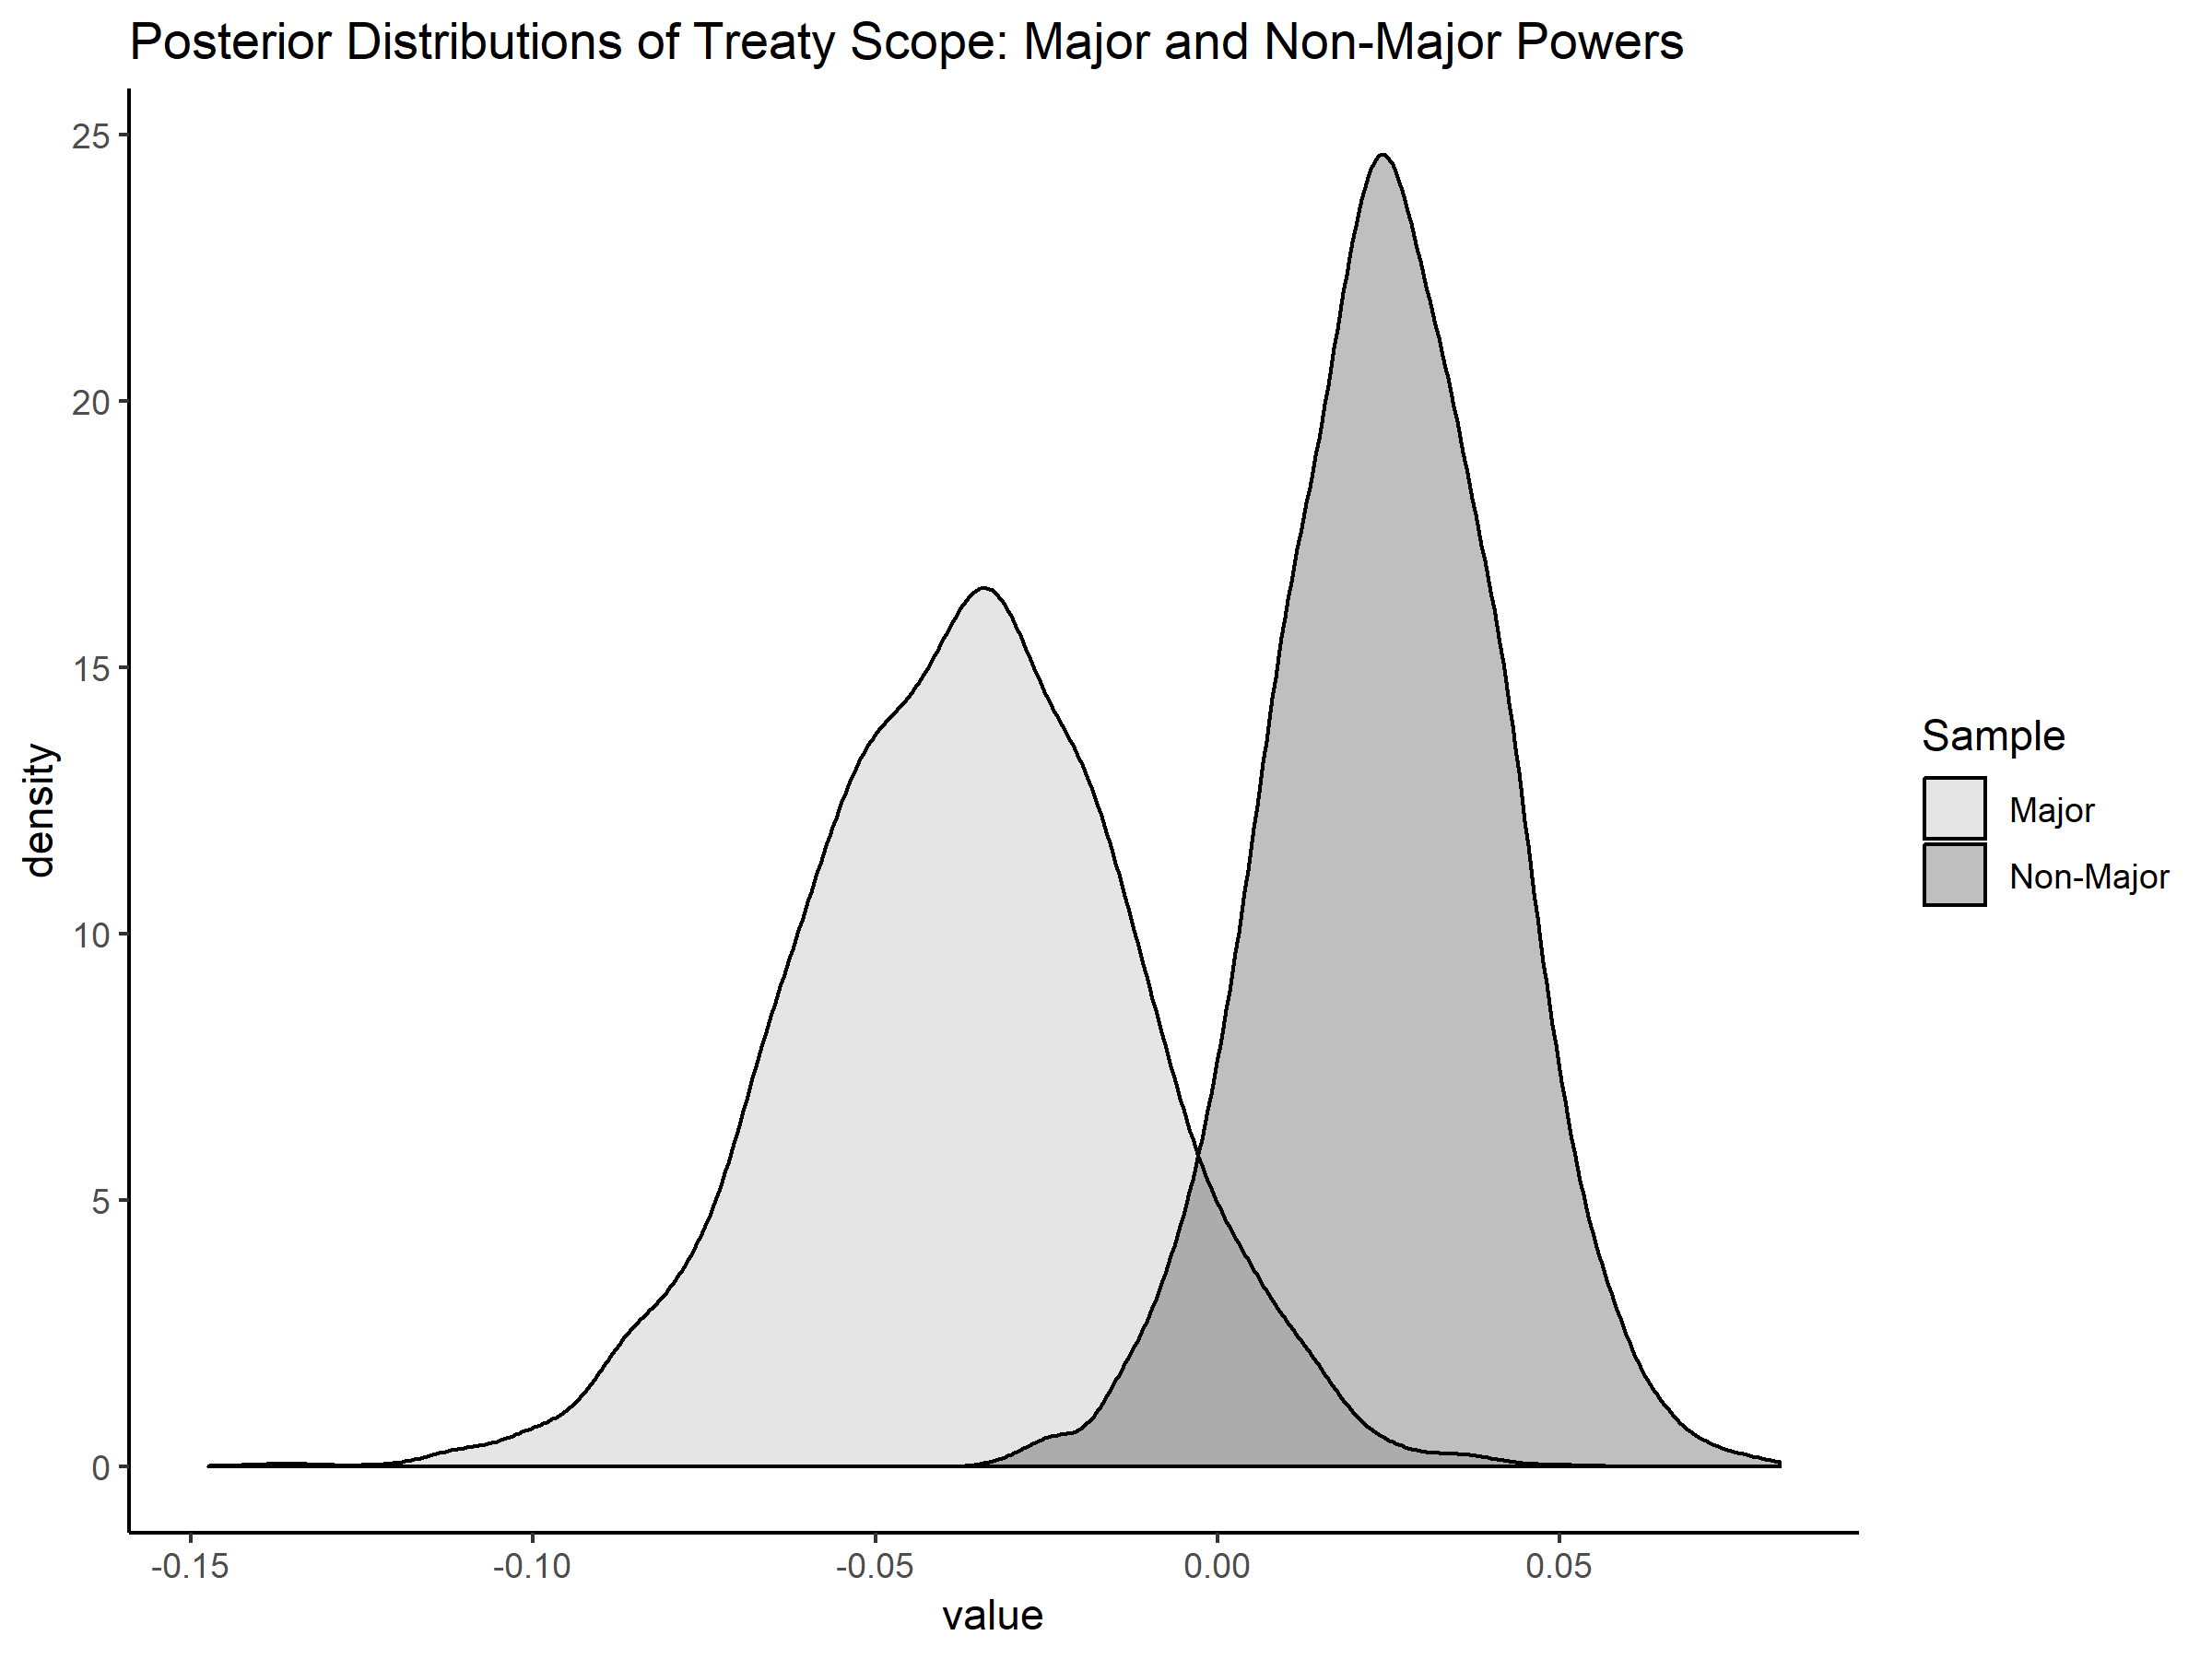
\includegraphics[width=0.95\textwidth]{scope-dens-joint.png}
	\caption{Posterior Distributions of Latent Scope in for major and non-major powers in a varying slopes model of alliance participation and military spending from 1816 to 2007. 94\% of the major power posterior mass is negative. 93\% of the non-major power posterior mass is positive.}
	\label{fig:scope-dens-joint}
\end{figure}


Because the varying slopes model shares information across major and non-major power groups, there is less uncertainty in the major power estimates in this model. 
Varying slopes also shrinks the major power posterior mean from -0.06 to -0.04, which indicates slightly smaller substantive effect of treaty scope. 
Even so, the amount of negative posterior mass is similar for major powers in the varying slopes and split samples. 


\autoref{tab:vary-slopes-alliance} summarizes the 90\% credible intervals for all the alliance level parameters. 
Again, the number of effective samples indicates little autocorrelation in the chains and $\hat{R}$ statistics suggest convergence. 


\begin{table}[ht]
\centering
\begin{tabular}{rrrrrrr}
  \hline
 & Mean & S.D. & 5\% & 95\% & Num. Eff. & $\hat{R}$ \\ 
  \hline
  Constant: Non-Major & -0.023 & 0.026 & -0.066 & 0.022 & 4000.000 & 1.000 \\ 
  Latent Scope: Non-Major & 0.025 & 0.017 & -0.003 & 0.051 & 4000.000 & 1.000 \\ 
  Number Members: Non-Major & 0.000 & 0.001 & -0.001 & 0.002 & 4000.000 & 1.000 \\ 
  FP Similarity: Non-Major & -0.011 & 0.025 & -0.053 & 0.029 & 4000.000 & 0.999 \\ 
  Democratic Membership: Non-Major & -0.002 & 0.001 & -0.005 & -0.000 & 4000.000 & 0.999 \\ 
  Wartime: Non-Major & 0.039 & 0.024 & -0.001 & 0.078 & 4000.000 & 1.000 \\ 
  Asymmetric: Non-Major & -0.030 & 0.022 & -0.066 & 0.007 & 4000.000 & 1.000 \\ 
  US Member: Non-Major & 0.010 & 0.018 & -0.019 & 0.040 & 4000.000 & 1.000 \\ 
  USSR Member: Non-Major & 0.016 & 0.040 & -0.051 & 0.083 & 4000.000 & 1.000 \\ 
  Constant: Major & 0.068 & 0.038 & 0.005 & 0.131 & 4000.000 & 1.002 \\ 
  Latent Scope: Major & -0.037 & 0.025 & -0.078 & 0.003 & 4000.000 & 1.000 \\ 
  Number Members: Major & -0.000 & 0.001 & -0.002 & 0.002 & 4000.000 & 1.000 \\ 
  FP Similarity: Major.1 & -0.059 & 0.034 & -0.116 & -0.004 & 4000.000 & 1.001 \\ 
  Democratic Membership: Major & -0.001 & 0.002 & -0.004 & 0.002 & 4000.000 & 1.000 \\ 
  Wartime: Major & -0.043 & 0.028 & -0.091 & 0.003 & 4000.000 & 1.000 \\ 
  Asymmetric: Major & 0.022 & 0.023 & -0.015 & 0.061 & 4000.000 & 1.001 \\ 
  US Member: Major & -0.009 & 0.027 & -0.056 & 0.035 & 4000.000 & 1.001 \\ 
  USSR Member: Major & 0.001 & 0.023 & -0.039 & 0.039 & 4000.000 & 0.999 \\ 
   \hline
\end{tabular}
\caption{90\% Credible intervals of alliance-level parameters in varying slopes model.}
\label{tab:vary-slopes-alliance}
\end{table}

  
\bibliography{../../MasterBibliography} 




\end{document}
